\documentclass[twocolumn]{article} % A4 paper and 11pt font size

\usepackage{lipsum} % Used for inserting dummy 'Lorem ipsum' text into the template
\usepackage[english]{babel} % English language/hyphenation
\usepackage[protrusion=true,expansion=true]{microtype} % Better typography
\usepackage{amsmath,amsfonts,amsthm} % Math packages
\usepackage{algorithm}
\usepackage{algpseudocode}
\usepackage[svgnames]{xcolor} % Enabling colors by their 'svgnames'
\usepackage[hang, small,labelfont=bf,up,textfont=it,up]{caption} % Custom captions under/above floats in tables or figures
\usepackage{booktabs} % Horizontal rules in tables
\usepackage{fix-cm} % Custom font sizes - used for the initial letter in the document
\usepackage{float}
\usepackage{bookmark}
\usepackage{enumitem}
\usepackage[parfill]{parskip}
\usepackage{minted} 
\usepackage{multicol}
\usepackage{caption}
\captionsetup{justification=raggedright}
\usepackage{graphicx} % Package to insert images
\graphicspath{ {./images/} }

\usepackage{sectsty} % Enables custom section titles
\allsectionsfont{\usefont{OT1}{phv}{b}{n}} % Change the font of all section commands

\usepackage{fancyhdr} % Needed to define custom headers/footers
\pagestyle{fancy} % Enables the custom headers/footers
\usepackage{lastpage} % Used to determine the number of pages in the document (for Page X of Total)

% Headers of all the pages - all currently empty
\lhead{}
\chead{}
\rhead{}

% Footers of all the pages
% \lfoot{}
\cfoot{\thepage}
\rfoot{\footnotesize Page \thepage\ of \pageref{LastPage}} % Format for Footnote: Page 1 of 2
\renewcommand{\headrulewidth}{0.0pt} % No header rule
\renewcommand{\footrulewidth}{0.4pt} % Thin footer rule

\usepackage{lettrine} % Package to accentuate the first letter of the text
\newcommand{\initial}[1]{ % Defines the command and style for the first letter
\lettrine[lines=3,lhang=0.3,nindent=0em]{
\color{DarkGoldenrod}
{\textsf{#1}}}{}}


%----------------------------------------------------------------------------------------
% TITLE SECTION
%----------------------------------------------------------------------------------------

\usepackage{titling} % Allows custom title configuration

\pretitle{\vspace{-30pt} \begin{flushleft} \fontsize{35}{35} \usefont{OT1}{phv}{b}{n} \selectfont} % Horizontal rule before the title

% Title here
\title{Deep Learning - Generative Adversarial Text to Image Synthesis} 
\posttitle{\par\end{flushleft}\vskip 2.0em} % Whitespace under the title
\preauthor{\begin{flushleft}\large \lineskip 0.0em \usefont{OT1}{phv}{m}{sl} \color{Black}} % Author font configuration
% Author here
\author{Alex Valle (4854159)   Gabriele Berruti (4791919)}
\postauthor{\footnotesize \lineskip 1em \usefont{OT1}{phv}{m}{sl} % Configuration for the institution name
% Add other iformations here if needed
\par\end{flushleft}} % Horizontal rule after the title
\date{} % Add a date here
%----------------------------------------------------------------------------------------

\begin{document}
\maketitle % Print the title
\thispagestyle{empty} % Enabling the custom headers/footers for the second page forward


%\section*{Abstract}

%Il Paper che si è deciso di analizzare è un documento risalente al 
%2016 che mostra lo sforzo di 6 ricercatori provenienti dall'Università 
%del Michigan e di Saarbrucken (Germania) . 
%Il documento mostra come l'utilizzo delle GAN (Generative Adversial Newtworks)
%permette un avanzamento nella generazione di immagini sintetiche partendo 
%da una descrizione testuale . 
%Esso mette a confronto il metodo proposto dalla ricerca e le 
%precedenti architetture che per quanto lontane dal traguardo descritto 
%sono in grado di ottenere rappresentazioni di feature testuali valide . 
%In particolare il paper vuole mostrare l'efficaccia del modello nel 
%generare immagini di uccelli e fiori partendo da una precisa descrizione 
%testuale degli stessi .
The paper that has been chosen for analysis is a document from 2016 
that showcases the effort of six researchers from the University of 
Michigan and Saarbrücken (Germany). 
The document shows how the use of GANs (Generative Adversarial Networks) 
allows for advancements in the generation of synthetic images starting 
from a textual description. 
It compares the method proposed by the research with previous architectures
that, although far from the described goal, are capable of obtaining 
valid textual feature representations. 
In particular, the paper aims to demonstrate the effectiveness of 
the model in generating images of birds and flowers based on a precise 
textual description of them.

\section*{Introduction}

In 2016, the ability of an AI system to generate realistic and 
coherent images from textual descriptions 
(such as "small red bird with a blue beak") was a current issue and 
far from being achieved.
It should be noted that it's necessary to use natural language 
and domain-specific attributes to describe the image to be generated.


 \subsection*{Related Papers Architectures}
 This paper is based on 3 documents that serve as a starting 
 point and tools for the proposed model:
 \begin{itemize}[noitemsep]
    \item \texttt{(Farhadi et al., 2009; Kumar et al., 2009;
    Parikh \& Grauman, 2011; Lampert et al., 2014)}: 
    3 Useful Papers for Encoding Distinctive Features of Objects 
    into Vectors (such as attributes used to distinguish 
    between different classes of objects)
    \item \texttt{(Fu et al., 2014 ; Akata et al., 2015)}: 
    2 Papers on "zero-shot" recognition, that is, recognizing 
    objects that have never been seen during the model's training.
    \item \texttt{(Yan et al., 2015).}: 
    And in Yan's paper, they discuss conditional image generation 
    in a manner similar to the method proposed here.
    \item \texttt{ (Reed et al., 2016)}: 
    Reed's paper presents highly discriminative and generic
    "zero-shot" text representations, 
    which are learnt automatically from words and characters.
\end{itemize}

\subsection*{Datasets}

\begin{itemize}[noitemsep]
    \item \texttt{Caltech-UCSD birds database (Wah et al., 2011)} : 
    Dataset used in related Papers previously described 
\end{itemize}

\subsection*{How to reach the goal ?}
The difficulty of translating words into images may be 
divided into two subproblems.
\begin{itemize}[noitemsep]
    \item \texttt{1.} : 
    First, learn a feature vector from a specific text 
    based on the visualization we want to obtain .
    \item \texttt{2.} : 
    Given these features through the use of a certain architecture, 
    create a realistic and coherent image.
\end{itemize}

\section*{Summary}

%Il Paper che si è deciso di analizzare è un documento risalente al 
%2016 che mostra lo sforzo di 6 ricercatori provenienti dall'Università 
%del Michigan e di Saarbrucken (Germania) . 
%Il documento mostra come l'utilizzo delle GAN (Generative Adversial Newtworks)
%permette un avanzamento nella generazione di immagini sintetiche partendo 
%da una descrizione testuale . 
%Esso mette a confronto il metodo proposto dalla ricerca e le 
%precedenti architetture che per quanto lontane dal traguardo descritto 
%sono in grado di ottenere rappresentazioni di feature testuali valide . 
%In particolare il paper vuole mostrare l'efficaccia del modello nel 
%generare immagini di uccelli e fiori partendo da una precisa descrizione 
%testuale degli stessi .
The paper that has been chosen for analysis is a document from 2016 
that showcases the effort of six researchers from the University of 
Michigan and Saarbrücken (Germany). 
The document shows how the use of GANs (Generative Adversarial Networks) 
allows for advancements in the generation of synthetic images starting 
from a textual description. 
It compares the method proposed by the research with previous architectures
that, although far from the described goal, are capable of obtaining 
valid textual feature representations. 
In particular, the paper aims to demonstrate the effectiveness of 
the model in generating images of birds and flowers based on a precise 
textual description of them.

\section*{Introduction}

In 2016, the ability of an AI system to generate realistic and 
coherent images from textual descriptions 
(such as "small red bird with a blue beak") was a current issue and 
far from being achieved.
It should be noted that it's necessary to use natural language 
and domain-specific attributes to describe the image to be generated.


 \subsection*{Related Papers \& Architectures}
 This paper is based on 3 documents that serve as a starting 
 point and tools for the proposed model:
 \begin{itemize}[noitemsep]
    \item \texttt{(Farhadi et al., 2009; Kumar et al., 2009;
    Parikh \& Grauman, 2011; Lampert et al., 2014)}: 
    3 Useful Papers for Encoding Distinctive Features of Objects 
    into Vectors (such as attributes used to distinguish 
    between different classes of objects)
    \item \texttt{(Fu et al., 2014 ; Akata et al., 2015)}: 
    2 Papers on "zero-shot" recognition, that is, recognizing 
    objects that have never been seen during the model's training.
    \item \texttt{(Yan et al., 2015).}: 
    And in Yan's paper, they discuss conditional image generation 
    in a manner similar to the method proposed here.
    \item \texttt{ (Reed et al., 2016)}: 
    Reed's paper presents highly discriminative and generic
    "zero-shot" text representations, 
    which are learnt automatically from words and characters.
    \item \texttt{(Goodfellow et al., 2014) \& (also studied
    by Mirza \& Osindero (2014) and Denton et al. (2015) )}: 
    Paper on application of conditional multi-modality for generative adversarial networks 

    \item \texttt{LEARNING A SHARED RAPPRESENTAZIONE ACROSS MODALITIES (MULTI-MODAL):}

    \item \texttt{Ngiam et al. (2011)}: 
    trained a stacked multimodal autoencoder on audio and video inputs and achieved a shared 
    modality-invariant representation.

    \item \texttt{Srivastava \& Salakhutdinov (2012)}: 
    developed a deep Boltzmann machine and jointly modeled images and text tags

    \item \texttt{Sohn et al. (2014) }
    proposed a multimodal conditional prediction framework

    \item \texttt{DEEP CONVOLUTIONAL DECODER NETWORK ARCHITECTURE :}
    
    \item \texttt{Dosovitskiy et al. (2015) \& Yang et al. (2015)}
    Used a deconvolutional network (with many layers of convolution and upsampling) 
    to create 3D chair representations based on shape, location, and illumination.
    And Yan added an encoder network to this approach .
    They trained a recurrent neural encoder-decoder to rotate 3D chair models
    and human faces based on rotational action sequences.

    \item \texttt{Reed et al. (2015)}
    Used a convolutional decoder to predict visual parallels between forms, video game characters, and 3D automobiles.

    \item \texttt{Goodfellow et al. (2014)}
    Introduced generative adversarial networks (GANs) and showed how GANs benefit from convolutional decoder networks for the generator module.

    \item \texttt{GENERATIVE ADVERSIAL NETWORK ....}
    
    \item \texttt{Denton et al. (2015)}
    Used a Laplacian pyramid of adversarial generators and discriminators to synthesize images 
    at multiple resolutions, producing high-resolution images and allowing generation conditioned on class labels

    \item \texttt{Radford et al. (2016)}
    Developed a stable and effective GAN architecture using a standard convolutional decoder, 
    incorporating batch normalization to improve image synthesis quality.

    \item \texttt{MULTI-MODAL LEARNING  }


    \item \texttt{Vinyals et al. (2015), Mao et al. (2015), Karpathy \& Li (2015), Donahue et al. (2015):}
    Introduced the use of recurrent neural network (RNN) decoders to generate text descriptions conditioned on images.

    \item \texttt{Hochreiter \& Schmidhuber (1997): }
    Used Long Short-Term Memory (LSTM) networks conditioned on top-layer features of deep convolutional networks 
    to generate image captions, especially with datasets like MS COCO.

    \item \texttt{Xu et al. (2015): }
    Incorporated a recurrent visual attention mechanism to further improve the results of text generation from images.

    \item \texttt{Ren et al. (2015) :}
    Generated replies to inquiries concerning picture visual content.

    \item \texttt{Wang et al. (2015) :}
    Expanded on Ren et al.'s technique by including an explicit knowledge foundation in the replying process.

    \item \texttt{Zhu et al. (2015) :}
    Used sequence models to align text (from books) and movies, allowing for simultaneous alignment of both.

    \item \texttt{Mansimov et al. (2016) :}
    Created pictures from text captions using a variational recurrent autoencoder with attention, 
    comparable to the DRAW model, which synthesized images in many stages.

    \item \texttt{Gregor et al. (2015) :}
    Created the DRAW model, which influenced Mansimov's way of producing graphics step by step.
    And obtaining realistic result also with "zero-shot" descriptions showing generalization . 

    \item \texttt{}
    \item \texttt{}


\end{itemize}



\section*{Datasets}
Bird and Flower images from human-written descriptions .

\begin{itemize}[noitemsep]
    \item \texttt{Caltech-UCSD Birds Database (Wah et al., 2011) ( CUB )} : 
    Dataset used in related Papers previously described and in this one as well .
    \item \texttt{Oxford-102 Flowers Dataset}
    Dataset used in this paper that correspond to have 5 text descriptions per image .
    \item \texttt{Test Dataset - MS COCO Dataset (Lin et al., 2014)}
    In addition to birds and flowers more general images and text descriptions .
\end{itemize}

\section*{How to reach the goal ?}
The difficulty of translating words into images may be 
divided into two subproblems.

\begin{itemize}[noitemsep]
    \item \texttt{1.} : 
    First, learn a feature vector from a specific text 
    based on the visualization we want to obtain .
    \item \texttt{2.} : 
    Given these features through the use of a certain architecture, 
    create a realistic and coherent image.
\end{itemize}
\section*{Effective Problems}
The paper highlights an intrinsic problem: when trying to generate images from textual descriptions, 
there are many different configurations that can be correct. ( Multi-modal Problem ). 
And even the reverse task, that is, generating descriptions from images, is difficult, 
but it is easier because it can be handled by predicting one word at a time, 
based on what has already been generated and the image itself.


\section*{Current Paper innovation ? }
Our technique differs from previous conditional GANs by focusing on text descriptions rather than class labels. 
This is the first design capable of differentiating from character to pixel level. 
The paper develop a manifold interpolation regularizer for the GAN generator, 
which enhances sample quality, including "zero-shot" categories on CUB.
It describes a model that generates 64x64 visually convincing pictures from text using a GAN. 
It differs from other models that just employ GANs for post-processing.
In practice it used a character-level text encoder and class-conditional GAN and 
focus in implementing a new architecture and using it on fine-grained  
image datasets described before ( CUB and Oxford Flowers ) .
Testing on MOCO dataset and test set disjoint from Training set 
can return a strong indicator on the performance of the system .


\section*{Background Knowledge}

\subsection*{
    GAN
}
The GAN architecture consist of two principal component :
Generator (G) and Discriminator (D) .
The main goal of D is to distinguish between real training images and generated images coming 
from G .
The idea is to maximize the logaritm of the loss of the Discriminator sampling images both from training set and 
generated while at the same time minimizing the outcoming of the log of 1 minus the loss of the Discriminator which has 
as input the generated image from random noise .

%  Log function 

\begin{figure}[h!]
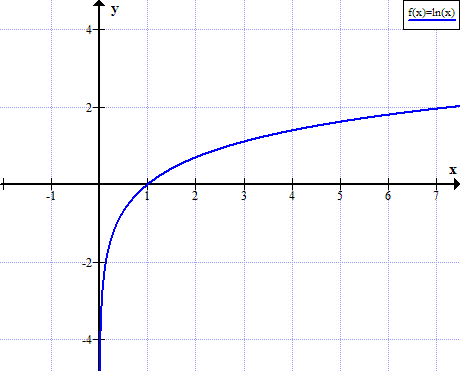
\includegraphics[width=80mm]{log.png}
\caption{Log Function}
\end{figure}
The Log function has a domain and an image that ranges from 0 to $\infty$.
It is possible to see that when the argument of the function tends to zero, the limit tends to -$\infty$, 
and when the argument tends to +$\infty$, the limit also tends to +$\infty$.

% Formula 
\subsection*{Formula}
\begin{equation}
    \min_{G} \max_{D} V(D, G) = \mathbb{E}_{x \sim p_{\text{data}}(x)}[\log D(x)] 
\end{equation}
\[
+ \mathbb{E}_{z \sim p_z(z)}[\log(1 - D(G(z)))]
\]
\begin{itemize}
    \item $D(x)$: the Discriminator as output layer use the Sigmoid function which map the data in a
    range from 0 to 1 .
    \item $G(x)$: the Generator instead as output layer use the Tanh function which map the data in a
    range from -$\infty$ to $\infty$ .
\end{itemize}

Therefore, based on these outputs and the behavior of the log function, it is possible to understand why 
the generator is minimized and the discriminator is maximized in the formula.
\\\\
So in detail the log function of the first expected value must have as arguments elements between 0 and 1 at most 
(output of D), therefore the first part of the equation, trying to maximize D, sees mainly negative values and at 
most equal to 0. \\
At the same time, the second equation with the second expected value calculates the difference between [ 1 - D(G(z)) ] 
, and since the argument of D tends to -infinity and we are simultaneously trying to maximize D and minimize G, 
the difference will result in a value between 0 and 1 (always positive).
Therefore, the limit of the logarithm as it approaches 0 will be equal to -$\infty$, 
while if the argument is 1, then the result is zero. \\
It's also possible to maximize G and use the log( [ D(G(z)) ] ) equation instead of log( [ 1 - D(G(z)) ] ) and 
obtain the same result . 


\subsection*{
    Text Encoder and Image Encoder via CLIP
}
To obtain a vector representation of text descriptions the main paper used the approch 
of Reed in 2006 using Deep convolutional and simmetric architecture based on both 
images a its corresponding text description . \\
The main idea in to have a dataset (Training set ) composed of N elements : 
\\
$ \{(v_n, t_n, y_n) : n = 1, ..., N\} $
\\
in which :
\begin{itemize}
    \item $ v_n $: correspond to the N images
    \item $ t_n $: correspond to the N text description
    \item $ y_n $: correspond to the class label ( usually there are more than two usually M )
\end{itemize}

First of all the paper define the classifier for both images and text description :
\begin{equation}
    f_v(v) = \arg \max_{y \in \mathcal{Y}} \mathbb{E}_{t \sim \mathcal{T}(y)} [\phi(v)^T \varphi(t)]
\end{equation}
    
\begin{equation}
    f_t(t) = \arg \max_{y \in \mathcal{Y}} \mathbb{E}_{v \sim \mathcal{V}(y)} [\phi(v)^T \varphi(t)]
\end{equation}

So in the first equation from all the possible class labels ($y$) we are trying to find the one that maximize the correlation between 
the input image and all the text descriptions on all the classes . \\
To do it we compute the multiplication between the encoded version of the input image $v$ and the current text description ($t$)
related to the current class . \\
In practice $\phi(v)$ and $\varphi(t )$ return a vector and we compute the similarity via a vector multiplication that return a scalar .\\ 
To compute the expected value in practice we compute the mean of all the scalar that we obtain from 
this multiplication on the specific class ($y$) .\\
In the second equation the formula is similar but on the input text description ($t$) .
The main idea was that an encoded description should have an higher compatibility 
with the images related to its class and so obtain higher value 

\begin{itemize}
    \item $\mathcal{Y}$: Set of the classes in which the images are divided .
    \item $\mathcal{T}(y)$: Set of the text description related to the $y$ class .
    \item $\mathcal{V}(y)$: Set of the images related to the $y$ class .
    \item $f_v(v)$: Classifier based on the images which return the class with higher compatibility with the image $v$
    \item $f_t(t)$: Classifier based on text description which return the class with higher compatibility with the description $t$
    \item $\phi(v)$: Image Encoder rappresentation on $v$ already trained on different dataset which return a vector (es. Obtained via CNN ).
    \item $\varphi(t)$: Text Encoder rappresentation on $t$ already trained on different dataset which return a vector (es. Obtained via CNN or LSTM).
    \item $\Delta$: Hinge or 0-1 loss for classification defined in which if the argument is higher than 0 it return 0 or 1 otherwise
    \item $\mathbb{E}_{t \sim \mathcal{T}(y)}$: Expected value in which $t$ correspond to all the text description related at the $y$ class .
    \item $\mathbb{E}_{v \sim \mathcal{V}(y)}$:  Expected value in which $v$ correspond to all the images related at the $y$ class .
\end{itemize}

Hinge or 0-1 Loss in this case is:

\begin{equation}
    \Delta( y, f(x) ) = max (0 , 1 - y * f(x) )
\end{equation}



\begin{equation}
    \varphi_{loss} = \frac{1}{N} \sum_{n=1}^{N} \Delta(y_n, f_v(v_n)) + \Delta(y_n, f_t(t_n)) 
\end{equation}

The main idea to compute the $\varphi_{loss}$ loss function was to learn the weights of 
the Text Encoder ($\varphi$) and fine-tuning it on our dataset .

During our implementation part this fine-tuning part has been done using 
the CLIP (Contrastive Language-Image Pre-Training) Text Encoder on the 
complete CUB and Flower dataset , in such a way to obtain 
relevant vector rappresentation which is composed of values that ranges 
from negative to positive values .


\section*{ Methodologies }
All the methods are based on a GAN architecture with a Generator G 
and a Discriminator D . \\ 
And use ($\varphi$) as Text Encoder that is a character-level convolutional-
recurrent neural network .

The generator is defined as :
\[
G : \mathbb{R}^Z \times \mathbb{R}^{T} \rightarrow \mathbb{R}^D,
\]
And the discriminator is defined as :  
\[
D : \mathbb{R}^D \times \mathbb{R}^{T} \rightarrow \{0, 1\},
\]
where 
\begin{itemize}
    \item ${D}$: is the dimension of the generated image
    \item ${Z}$: is the dimension of the input noise 
    \item ${T}$: is the dimension of the text emdedded with $\varphi$
\end{itemize}

\subsection*{- Generator Part -}
First of all the generated image is defined as :
\[
\hat{x} \leftarrow G(z, \varphi(t))
\]
This Generator take as input a noise vector of dimension Z 
(In our implementation Z = 100) whose values are sampled from a Gaussian 
distribution between 0 and 1
\\
\[
z \in \mathbb{R}^Z \sim \mathcal{N}(0, 1)
\]
and the vector coming from the Text Encoder $\varphi$ for the specific 
text description t obtaining $\varphi(t)$ .
\\
First part - Projection \\
The first step of the Generator Net is to reduce the dimension of 
$\varphi(t)$ using one fully-connected layer to project 
to the dimension of the projection P . \\
This part continue using a Normalization Layer (BatchNorm1d)
and a Leaky-Relu as activation function with a specific negative slope .  
So the values on the vector can be negative and positive depending on the 
situation .

In our implementation $\varphi$ correspond to CLIP while \\
T is equal to 512 and \\
P is equal to 128 \\
After this first part an 128-dim vector is obtained and defined as :
\[
 p = projection( \varphi(t) )
\]

Second part - Concatanation \\
To compose the Latent Space vector (LSV) the paper suggested to concatenate 
the noise vector z with the projected vector p .

In our specific implementation the latent space has a dimension of H (H=228)
which is simple the concatation of the two vector of dimension T=100 
and P=128 .

\[
h = concat( z , p )
\]

Third part - Final Net to generated the image 64x64 RGB 
As input of the Final Net part of the Generator is the Latent Space Vector 
(LSV) of dimension H (H=228). 

This Final Net is composed of 4 set of layers in which the first one is a 
Convolutional Transpose 2D Layers ( "to up-sample" ) followed by a Normalization layer 
and Relu as activation function so we only have values greater than 0 .

In our implementation the initial dimension of the vector was (228,1,1) but 
after only the first Convolutional Transpose layer it is projected into an higher dimension of 
(512,8,8) .

After using the other 3 set of layers the dimension will be equal to (64,32,32) .
The last layer is useful because permit to obtain an image of the shape 
(3,64,64) and is composed of a Convolutional Transpose 2D Layer and Tanh as activation function .

Using Tanh with in input values coming from the last layer that can be positive and 
negative as well due to the weight of the 2D Convolutional Transpose Layer we will obtain an 
image 64x64 with 3 channel RGB with values that ranges from -1 to 1 due to Tanh .
\[
\hat{x} = generate( h )
\]
And G is defined as this 3 Parts applied in order one after another  . 


\subsection*{- Discriminator Part -}
The Discriminator is defined as this :
\[
D ( \hat{x} , \varphi(t) ) = \left\{ x_i \in [0, 1] \mid i = 0, 1, \dots, 120 \right\}
\]
It takes in input the generated image $\hat{x}$ and depending
on the situation an encoded version of the text description $\varphi(t)$
related or not to image generated .

Similarly to what we have seen in the Generator Part the Discriminator is 
sub-divided in 3 Parts or Networks . 

First Net - Down-Sampling 
The First Part is composed of a several (in our implementation 4) set 
of Convolutional 2D Layers ("to down-sample") 
followed by a normalization Layer (BatchNorm2d except the first set)
and Leaky-Relu as activation function . 
After passing through this Net the generated image of a shape of (3,224,244)
will have a dimension of (512,14,14) .
\[
 q = DownSampling( \hat{x} )
\]

Second Part - Projection Text Emdedding and Concatenation

This part consist of two phases and it take as argument the down-sampled generated 
image ${q}$ and the encoded version of the text description $\varphi(t)$ .
The first phase consist in projecting $\varphi(t)$
in a lower-dimension P (P=128) using one fully-connected layer and normalization layer 
followed by a Leaky-Relu as activation function in the exact same way that we have done in 
the Generator .
After this first phase a 128-dim vector is obtained and defined as :
\[
 p = projection( \varphi(t) )
\]
The last task of the first phase was to adapt the project dimension of p 
( that is (128,1,1) ) in such a way to be compatibile with the second phase 
which concatenate p with q . 
So the dimension of p is squeezed into a dimension that allow to concatenate
the two data and it became (128,14,14)
\[
 \hat{p} = squeeze( p )
\]

The second Phase consist of the concatenation of $q$ and $\hat{p}$ 
which result in a dimension of (512+128, 14, 14) = (256, 640, 14, 14)
This concatation permit to obtain the Latent vector c :
\[
 c = concatenate( q , \hat{p} )
\]


Third Part - Final Net 
This Final Net it's only composed of One Convolutional 2D Layer and 
Sigmoid as activation function which map the input in a range that goes 
from 0 to 1 .
The first Convolution Layer modify the shape from (256, 640, 14, 14) 
to (512,4,4) while the sigmoid function change its shape into
( 1,11,11 ) .
At the end of this phase we flatten the 11x11 values into a vector of 
121-dimension .
So at the end for each generated image and text Emdedding we obtain a 
121-dim vector rappresenting the discriminator factors .
\[
 d\_loss = FinalNet( c )
\]

--------------------------


\section*{Architectures}

\subsection*{(Vanilla GAN) :  Generative Adversarial Network without Conditional Latent Space }
The Vanilla implementation stands for an implementation in which the Generator only depend 
on the noise vector z and not depend on the Conditional Latent Space $ \varphi(t) $ and the same 
stand for the discriminator which depends only on the actual or the generated image .

\subsection*{(GAN-CLS) :  Generative Adversarial Network with Conditional Latent Space }
The idea behind this architecture is to use $\varphi$ as Text Encoder (CLIP)
to create the embeddings related to text description ${t}$ coeherent with the image (${x}$) 
to obtain ${h}$ and one not correlated to the image sampled randomly $\hat{t}$ to obtain $\hat{h}$ .
Another step is to generate the Noise Vector ${z}$ randomly sampled from a Gaussian 
Distribution . \\
The following step is to generate an image passing through ${z}$ and ${h}$ as explained 
in the Generator Part and otbaining $\hat{x}$ .
As well the Discriminator have to compute a value ${s_r}$ that correspond to 
the loss passing through it the real image ${z}$ and the corresponding text 
emdedding ${h}$ . \\
In the same way we obtain ${s_r}$ passing at inference time 
the image ${x}$ and $\hat{t}$ and we calculate 
${s_f}$ passing the image ${x}$ and ${h}$ . 
The Final part consist in computing the Discriminator loss $L_D$ as the 
$\log(s_r) + \left(\log(1 - s_w) + \log(1 - s_f)\right) / 2$ . \\
In the actual implementation the loss of the Discriminator is computed 
using the BCELoss (Binary Cross Entroy Loss) between ${s_r}$ and a 
"smoothed" version of the label filled with 1 computing "${d\_loss\_r}$" and again two times , first 
with ${s_f}$ and a "fake label" filled with 0 computing "${d\_loss\_f}$" and after using 
${s_f}$ and the "fake label" computing "${d\_loss\_f}$" . \\
So the final value is computed summing the 3 obtained values :
\[
 L_D = d\_loss\_f + d\_loss\_w + d\_loss\_r
\]
After this computation the Discriminator is updated using backpropagtion 
based on the gradient with $\alpha$ as parameter .

For the Generator Loss $L_D$ we don't compute only the logarithm
of ${s_f}$ (\ in Algorithm 1 )\ but we use a custom loss composed of 3 part .
The first one compute the BCELoss between ${s_f}$ and the "real label" which is
a vector filled with 1 . \\
The second one compute the MSELoss (\ Mean Squared Error Loss )\ between 
${q_r}$ (after Down-Sampling) and ${q_f}$ coming from the Discriminator of
${s_r}$ and ${s_f}$ . \\
The Third part is computed the L1Loss between the generated image $\hat{x}$
and the real image ${x}$ .
The 3 part are summed to obtain $L_G$
\[
 L_G = BCELoss( s_f,real\_label ) + MSELoss( q_r , q_f ) 
\]
\[
 + L1Loss(\hat{x},x)
\]
And finally after this computation the Generator is updated using backpropagtion 
based on the gradient with $\alpha$ as parameter .



\begin{algorithm}
    \caption{GAN-CLS training algorithm with step size $\alpha$, using minibatch SGD for simplicity.}
    \begin{algorithmic}
        \Require minibatch images $x$, minibatch matching text $t$, minibatch mis-matching text $\tilde{t}$, 
        number of training batches $S$
        \For{$n = 1$ to $S$}
            \State $h \leftarrow \varphi(t)$ \hfill \{Encode matching description\}
            \State $\hat{h} \leftarrow \varphi(\tilde{t})$ \hfill \{Encode mis-matching description\}\
            \State $z \sim \mathcal{N}(0, 1)^Z$ \hfill \{Extract Noise Vector\}
            \State $\hat{x} \leftarrow G(z, h)$ \hfill \{Forward through generator\}
            \State $s_r \leftarrow D(x, h)$ \hfill \{Real image, right text\}
            \State $s_w \leftarrow D(x, \hat{h})$ \hfill \{Real image, wrong text\}
            \State $s_f \leftarrow D(\hat{x}, h)$ \hfill \{Fake image, right text\}
            \State $L_D \leftarrow \log(s_r) + \left(\log(1 - s_w) + \log(1 - s_f)\right) / 2$
            \State $D \leftarrow D - \alpha \nabla L_D$ \hfill \{Update discriminator\}
            \State $L_G \leftarrow \log(s_f)$
            \State $G \leftarrow G - \alpha \nabla L_G$ \hfill \{Update generator\}
        \EndFor
    \end{algorithmic}
\end{algorithm}


\subsection*{(GAN-INT) :  Generative Adversarial Network Interpolated}
The main difference with respect with the previous implementation relies 
in the fact that Generation of the "fake image" do not depend not anymore 
only on z and t ,but in an interpolation of two different text emdeddings .
In practice the paper found that fixing ${\beta}$ = 0.5 works well and want to
underline that t1 and t2 may come from different images and 
even different categories.
This parte has not been implemented and tasted but with little modification
on the actual code can be performed . 


\begin{equation}
    \mathbb{E}_{h1,h2 \sim p_{data} } [\log( 1 - D(G( z , \beta h1 + 
    (1-\beta) h2 )))]
\end{equation}

\subsection*{- WGAN : - Wessertstain GAN}
This typology of GAN is not present in the Paper but follow the same concept 
described before . 
In principle we can observe first all the algorithm :

\begin{algorithm}
    \caption{WGAN training algorithm with step size $\alpha$, using minibatch SGD for simplicity.}
    \begin{algorithmic}
        \Require minibatch images $x$, minibatch matching text $t$, minibatch mis-matching text $\tilde{t}$, 
        number of training batches $S$ , number of iteraton for the Discriminator $NI$ 
        \For{$n = 1$ to $S$}
            \State $h \leftarrow \varphi(t)$ \hfill \{Encode matching description\}
            
            \For{$n = 1$ to $NI$}
                \State $z \sim \mathcal{N}(0, 1)^Z$ \hfill \{Extract Noise Vector\}
                \State $\hat{x} \leftarrow G(z, h)$ \hfill \{Forward through generator\}
                \State $s_r \leftarrow D(x, h)$ \hfill \{Real image, right text\}
                \State $s_f \leftarrow D(\hat{x}, h)$ \hfill \{Fake image, right text\}
                \State $L_D \leftarrow (s_r) - (s_f) $
                \State Clip weights of $D$ within $[-c, c]$
                \State \{Lipschitz constraint\}
            \EndFor
            \State $z \sim \mathcal{N}(0, 1)^Z$ \hfill \{Extract again Noise Vector\}
            \State $\hat{x} \leftarrow G(z, h)$ \hfill \{Forward through generator\}
            \State $s_f \leftarrow D(\hat{x}, h)$ \hfill \{Fake image, right text\}
            \State $L_G \leftarrow -(s_f) $ \hfill \{Wasserstein loss for Generator\}
            \EndFor
    \end{algorithmic}
\end{algorithm}

The idea behind this architecture is to use $\varphi$ as a Text Encoder to create embeddings 
related to a text description $t$ that matches the image $x$, obtaining $h$. 
This embedding $h$ serves as the condition for both the Generator and Discriminator. \\
Another step involves sampling a Noise Vector $z$ randomly from 
a Gaussian Distribution $\mathcal{N}(0, 1)^Z$. \\
The following step is to generate a fake image $\hat{x}$ by passing $z$ 
and $h$ through the Generator $G$. \\
The Discriminator $D$ computes a score $s_r$ by passing the real image $x$ and 
the corresponding text embedding $h$, which reflects how well $D$ recognizes 
the real data. \\
Similarly, the Discriminator computes a score $s_f$ by passing 
the generated image $\hat{x}$ and the same text embedding $h$.\\
The Discriminator loss $L_D$ is calculated as the difference $s_r - s_f$, which represents 
the Wasserstein distance. To enforce the Lipschitz constraint, the weights of 
the Discriminator are clipped within a fixed range $[-c, c]$ after every update. \\
This ensures the Discriminator satisfies the required gradient properties for stable training.
After training the Discriminator for multiple steps, the Generator is trained. \\
A new Noise Vector $z$ is sampled from $\mathcal{N}(0, 1)^Z$, and a fake image $\hat{x}$ 
is generated by passing $z$ and $h$ through $G$. \\
The Discriminator then computes a new score $s_f$ for this generated image, 
and the Generator loss $L_G$ is calculated as $-s_f$. \\
This encourages the Generator to produce images that maximize the Discriminator's score, 
effectively improving the quality of the generated images. \\
The training process alternates between optimizing the Discriminator and the Generator. 
Over multiple iterations, the Discriminator learns to distinguish real and fake images better, 
while the Generator learns to produce more realistic images. \\
This iterative process ensures that the Wasserstein distance between the real and generated 
data distributions is minimized, leading to stable and efficient GAN training.

\subsection*{Generator Inversion for Style Transfer}

The text encoding \(\varphi(t)\) represents the content of an image 
(e.g., flower shape and colors). 
To generate realistic images, the noise sample \(z\) should encode 
style elements such as background color and pose. 
Using a trained GAN, it becomes possible to transfer the style from 
a query image to align with the content of a specific text description.

This is achieved by training a convolutional network \(S\) to invert 
the generator \(G\), allowing the recovery of \(z\) 
from generated samples \(\hat{x} \leftarrow G(z, \varphi(t))\). 
The style encoder \(S\) is trained using a simple squared loss function:

\[
\mathcal{L}_{\text{style}} = \mathbb{E}_{t, z \sim \mathcal{N}(0, 1)} \| z - S(G(z, \varphi(t))) \|_2^2 \tag{6}
\]

Here, \(S\) denotes the style encoder network.

Once the generator and style encoder are trained, 
the style from a query image \(x\) can be transferred to match a text 
description \(t\) as follows:

\[
s \leftarrow S(x), \quad \hat{x} \leftarrow G(s, \varphi(t))
\]

In this process, \(s\) represents the extracted style, and \(\hat{x}\) 
is the final image output.

\section*{Experiments Are the experiments reproducible? What are the main insights from the experimental analysis?}

\section*{Experiment conducted by the Paper}

\subsection*{Datasets}

\subsubsection*{CUB Dataset}
The CUB dataset contains 11,788 bird images belonging to 200 distinct categories. 

\subsubsection*{Oxford-102 Dataset}
The Oxford-102 dataset consists of 8,189 flower images, grouped into 102 categories.

\subsubsection*{Data Splits}
For training and evaluation, datasets are split into class-disjoint subsets:  
\begin{itemize}
    \item \textbf{CUB:} 150 categories are used for training and validation, while the remaining 50 are used for testing.
    \item \textbf{Oxford-102:} 82 categories are assigned to training and validation, and 20 categories are reserved for testing.
\end{itemize}

\subsubsection*{Captions}
Each image in both datasets is accompanied by 5 captions. During training, a random image view (e.g., crop, flip) and one randomly selected caption are used for each mini-batch.

\subsection*{Text Encoder}

\subsubsection*{Encoder Architecture}
The text encoder employs a deep convolutional-recurrent network, combining a character-level ConvNet with a recurrent neural network (char-CNN-RNN). This architecture generates 1,024-dimensional embeddings for textual descriptions.

\subsubsection*{Text Embedding}
Text captions are embedded into a 1,024-dimensional space via structured joint embedding with GoogLeNet features. 

\subsubsection*{Pre-training}
Pre-training the text encoder accelerates the training of the generator and discriminator, enabling faster experimentation. While pre-training is not a strict requirement, end-to-end training results are provided in the supplement for completeness.

\subsubsection*{Generalization}
Qualitative results from the MS COCO validation set illustrate the approach's ability to generalize beyond the datasets used in training.

\subsection*{GAN Architecture}

\subsubsection*{Training Image Size}
All training images are resized to \(64 \times 64 \times 3\).

\subsubsection*{Text Feature Projection}
Text embeddings are projected to a 128-dimensional space before being concatenated with convolutional feature maps in both the generator and discriminator networks.

\subsubsection*{Training Process}
The generator and discriminator in the GAN-CLS architecture are updated 
in alternating steps to optimize the GAN architecture.

\subsubsection*{Hyperparameters}
The following hyperparameters are used during training:
\begin{itemize}
    \item Base learning rate: 0.0002.
    \item Optimizer: ADAM, with a momentum parameter of 0.5.
    \item Generator noise: Sampled from a 100-dimensional unit normal distribution.
    \item Mini-batch size: 64.
    \item Number of epochs: 600.
\end{itemize}

\subsubsection*{Implementation}
The implementation of the model is based on the \texttt{dcgan.torch2} 
framework.

\section*{Paper Qualitative Results}

\subsection*{Comparison of GAN Variants}

We compare the following GAN architectures:  
\begin{itemize}
    \item \textbf{GAN Baseline:} The basic GAN model without any specific improvements for text-image matching.  
    \item \textbf{GAN-CLS:} A GAN model incorporating an image-text matching discriminator .  
    \item \textbf{GAN-INT:} A GAN variant utilizing text manifold interpolation
    \item \textbf{GAN-INT-CLS:} A model combining both text manifold interpolation and the image-text matching discriminator.  
\end{itemize}

\subsection*{Results on the CUB Dataset}
Qualitative results for the CUB dataset:  
\begin{itemize}
    \item The \textbf{GAN Baseline} and \textbf{GAN-CLS} models correctly reproduce some color information. However, the generated images do not appear realistic.  
    \item \textbf{GAN-INT} and \textbf{GAN-INT-CLS} models produce plausible bird images that match either all or part of the captions.  
    \item Additional robustness analysis for each GAN variant on the CUB dataset is provided in the supplement.  
\end{itemize}

\subsection*{Results on the Oxford-102 Dataset}
Qualitative results for the Oxford-102 Flowers dataset are presented in Figure 4:  
\begin{itemize}
    \item All four models are capable of generating plausible flower images that align with their respective captions.  
    \item The \textbf{GAN Baseline} exhibits the highest variety in flower morphology, especially when the caption does not specify petal types.  
    \item Other models, such as \textbf{GAN-CLS}, \textbf{GAN-INT}, and \textbf{GAN-INT-CLS}, generate more class-consistent flower images.  
    \item It is speculated that generating flowers is easier than birds 
    due to structural regularities in bird species, making it simpler 
    for the discriminator to identify fake birds compared to fake flowers.  
\end{itemize}

\subsection*{Additional Results}
Supplementary materials include additional examples for the following:  
\begin{itemize}
    \item \textbf{GAN-INT} and \textbf{GAN-INT-CLS} models on both CUB and Oxford-102 datasets.  
    \item \textbf{Vanilla GAN:} An end-to-end variant of GAN-INT-CLS that does not rely on pre-training the text encoder \(\phi(t)\).  
\end{itemize}

\subsection*{Disentangling Style and Content}

This section explores the capability of the model 
to separate style from content. 
\\
By \textit{content}, we refer to the intrinsic visual 
characteristics of the bird, such as the shape, size, 
and color of its body parts. 
\textit{Style}, on the other hand, encompasses external 
factors like background color and pose orientation.
\\
Since the text embedding primarily encodes content 
information and usually excludes style details 
(e.g., captions rarely describe background or pose), 
the GAN must utilize the noise vector \(z\) 
to account for variations in style. 
\\
To generate realistic images, the disentanglement 
of these factors is crucial.
\\
To measure the extent of style-content disentanglement 
on the CUB dataset, we defined two tasks: 
\\
pose verification and background color verification. 
Each task required constructing pairs of similar and 
dissimilar images. 
Style vectors for these images were obtained by passing 
them through a style encoder network, 
trained to invert the generator's outputs back to the 
noise vector \(z\). 
\\
If style and content are disentangled, images with similar 
styles (e.g., same pose) should have higher similarity 
scores than images with different styles 
(e.g., different poses).
\\
To recover \(z\), we inverted the generator networks 
following the procedure in Subsection 4.4. Verification 
pairs were created by clustering images into 100 groups 
using K-means. For background color verification, 
clustering was performed based on the average RGB values 
of the background. 
\\
For pose verification, clustering relied on six keypoint 
coordinates (beak, belly, breast, crown, forehead, and tail).
\\
Evaluation was performed by calculating predicted style 
vectors for image pairs using style encoders for GAN, 
GAN-CLS, GAN-INT, and GAN-INT-CLS models. 
\\
Similarity scores were computed with cosine similarity, 
and the AU-ROC metric was reported, averaged over five 
folds. 
\\
As a baseline, cosine similarity between text features 
from the text encoder was also calculated.
\\
The results, shown in Figure 5, confirm that 
captions alone do not provide style-related information. 
Consistent with qualitative observations, models 
incorporating interpolation regularization 
(GAN-INT and GAN-INT-CLS) achieved superior performance 
for these tasks. \\
Specifically:

\begin{itemize}
    \item \textbf{Pose Verification:} ROC curves demonstrate 
    that style encoders effectively distinguish between 
    similar and different poses.
    \item \textbf{Background Color Verification:} ROC curves 
    illustrate that models can separate images based 
    on background color variations.
\end{itemize}


\subsection*{Pose and Background Style Transfer}

GAN-INT-CLS, when combined with a trained style 
encoder (as described in the Style Transfer 
subsection), enables style transfer from an unseen query 
image to a new text description. 
\\
Remarkably, this approach often retains intricate 
background details, such as a tree branch on which 
the bird is perched, showcasing the effectiveness
of disentangling style and content.
\\
The ability of GAN-INT-CLS to disentangle style is 
particularly noteworthy as it facilitates a 
straightforward method of generalization. 
\\
By leveraging this disentanglement, the model can 
combine previously observed content 
(e.g., text descriptions) with previously seen styles 
in novel pairings, thereby generating realistic 
and plausible images that are entirely distinct from 
those seen during training. 
\\
Another pathway for generalization involves utilizing 
attributes present in the training data
(e.g., "blue wings" and "yellow belly") to create new 
combinations. 
\\
\section*{Sentence Interpolation}

Although ground-truth text descriptions are not 
available for the interpolated points, 
the generated images appear visually coherent 
and plausible. 
\\
By holding the noise distribution constant, 
the only variable factor across each row is 
the text embedding. 
\\
This approach allows interpolations to accurately 
capture content-related changes, 
such as a bird transitioning from blue to red, 
while preserving consistent pose and background 
elements.
\\
In addition to sentence interpolation, 
Figure 8 (Right) presents results achieved 
through noise interpolation. 
\\
In this case, two random noise vectors are sampled, 
and by keeping the text embedding fixed, 
we interpolate between these noise vectors. 
\\
The resulting images display a smooth style 
transition while maintaining fixed content. 
\\
This demonstrates the model's ability to 
disentangle style and content effectively, 
enabling independent manipulation of each aspect 
to produce seamless variations in generated 
images.

\subsection*{Training on other dataset - MOCO}

To demonstrate the generalization capability of 
our approach, we trained a GAN-CLS model on the 
MS-COCO dataset. 
\\
We have to underline that unlike CUB and Oxford-102, 
MS-COCO features diverse images containing multiple 
objects and 
variable backgrounds. 
\\
Despite this complexity, we employed the same text encoder, GAN architecture, 
and hyperparameters (learning rate, mini-batch size, and number of epochs) 
used in the previous datasets. 
\\
The main difference lies in the text encoder training, as COCO lacks a single 
object category per class, requiring an instance-level image and text matching approach.
\\
Figure 7 displays examples of generated images alongside their corresponding 
ground-truth captions. 
\\
The results exhibit sharpness typical of GAN-based synthesis methods and 
notable diversity in samples, 
achieved by varying the noise vector while keeping the text embedding fixed.
\\
However, closer inspection reveals some limitations in scene coherence, 
particularly in complex scenarios like human figures in baseball scenes, 
where articulated parts are missing. 
\\
Future work could explore incorporating hierarchical structures into the 
synthesis model to better handle multi-object scenes.
\\
Additionally, a qualitative comparison with AlignDRAW (Mansimov et al., 2016) 
is provided in the supplement. 
\\
While GAN-CLS produces sharper and higher-resolution outputs roughly matching the query, 
AlignDRAW better captures fine-grained single-word variations. 
Extending the GAN-CLS generator network with temporal structures could improve
its ability to handle nuanced text differences.

\section*{Paper Conclusions}

This work presented a simple yet effective model for generating images 
from detailed visual descriptions. 
\\
Our approach successfully synthesized multiple plausible visual 
interpretations for a given text caption. 
\\
The introduction of a manifold interpolation regularizer significantly 
enhanced text-to-image synthesis on the CUB dataset. 
\\
We also demonstrated the ability to disentangle style and content, 
enabling bird pose and background transfer from query images 
to text descriptions. 
\\
Furthermore, our model showed generalizability to more complex scenarios, 
generating images with multiple objects and variable 
backgrounds on the MS-COCO dataset. 
\\
Future work will focus on scaling the model to produce higher-resolution 
images and incorporating a broader range of text inputs.


\newpage

\section*{Our Code implementation }
The code has been written in Python , while back in 2016 the researcher 
decided to write the code for training the Net in LUA .
So first of all we understand the code written in LUA by the authors and 
after we decide to translate it in Python . 
The main reason why we do it is that the code was deprecated after about 10 years (
especially the library ) and for us was not possible to try to train the Net 
ourself . 
Talking about the Datasets they were also not reacheable because the hyperlink redirect 
to a website not existing anymore .
So we try to develop a solution in which we train the Net with the same concept described 
before but using different Datasets .  
Also the trained weights cannot be adapted to the new solution that we develop ,
so we decide so re-train the Network from zero for about 200 epochs .
After the 200 epochs we decide to stop the training because it was taking too long .
\\
The code in subdivided in different part and diffent .ipynb file .
The first one is "1) dataset usage.ipynb" in which is possible the are two example 
on how to load Bird and Flowers Dataset using the module "gan\_t2i" and store it in HDF5 format 
other than using a Dataloader on this datasets .
The second file is "2) CLIP - Fine Tuning.ipynb" in which is shown how to load the CLIP model 
(ViT-B/32) and to train it (we use an already trained CLIP network to extract text features )
The Third file is "3.2) COLAB GAN example.ipynb" . In this file we combine all the 
module that we develop until now . 
First of all we decide which network we would like to train between : "Vanilla\ GAN", "GAN\_INIT\_CLS" 
and "WGAN" . 
After this part we download the weights related to the CLIP Network used to extract 
the text features and also the model itself .
What about the Dataset initially it is stored in HDF5 format but this time is also 
transformed and normalized other than tokenized .
After this section we create the training, validation and test dataloaders and check the 
outcome size of the CLIP model feature related to text and images .
And then depending on the Newtwork that we would like to train 
we define it and define the embedding projection dimension that in our case is 128 .
Finally after this long pre-processing and initilization part we can decide if start to train
the Net using the correspondent Algoritm from zero or from a specific checkpoint ( which corrispond
to the weights ) loading it in the Model . 
The result on the GAN model after 186 epochs of training from scratch are not enough to prodoce a result 
which correspond to the description given by the text , that's due to the fact that the Net is too complex 
and in fact to achieve a satisfactory result, at least 600 epochs are necessary, 
as the original paper also specifies.
Besides the visualization factor it's possible to observe that the loss related to the Discrimination and 
Generator part tend to move in the right direction , in fact the Generator loss especially in the WGAN model
tend do descrease (minimize) and the Discriminator loss it's maximizing it's values as well as described 
in the Min-Max optimization formula .
\\
\section*{WGAN on FASHION-MNIST Dataset}
We try also to conduce some experiments on training the Net addressing the problem to other Datasets 
such as Fashion MNIST dataset ( keras.datasets.fashion\_mnist ) .
\\
So in general the WGAN employs the Wasserstein distance 
to define a value function with properties theoretically superior  
compared to the one introduced in the original GAN paper .
As seen before to verify that the Discriminator (critic) respects the 
1-Lipschitz requirement, the authors implemented weight clipping. 
However, this technique might lead to problems like as low convergence 
in deep critics and other unwanted phenomena.
WGAN-GP substitutes weight clipping with a "gradient penalty." 
This variant includes a loss term to keep the L2 norm of the discriminator 
gradients around a set value, allowing for smoother training . But it's based 
on the Algoritm \ref{alg:WGAN} flow-chart described in the section related to the 
Architectures.
\\
\subsection*{Data Preparation}
The dataset used is the FASHION-MNIST dataset , in which each 
sample is a 28x28 grayscale pixel image with values 
normalized in the range [-1,1] . 
The label related to the image will not be used in this case 
to train the WGAN .
\\
\subsection*{Discriminator Net}
In this case the Discriminator use a Zero Padding layer to transform 
the input image (28,28,1) into a shape of (32,32,1) and other
4 Convolutional Block to transform it in (16,16,64) $\rightarrow$  ( 8, 8, 128)
$\rightarrow$ (4, 4, 256) $\rightarrow$ (2, 2, 512)
Leaky Relu is used as activation function .
\\
The Convolutional Block is composed of 2D Convolutional Kernel 
and depending on the parameters a Normalization and dropout layer .
The output shape of the discriminator is one value that rappresent 
the "real" or "fake" classification of the input image, 
indicating whether the image is from the real dataset or 
generated by the Generator.
\subsection*{Generator Net} 
The Genetor Net use the upsample\_block(..) function 
to handle the upsampling process by increasing the spatial 
dimensions of the input with UpSampling2D, followed by a Conv2D layer .
Depending on the parameter it may also include BatchNormalization 
and a specific activation function (like LeakyReLU or Tanh) 
to introduce non-linearity and improve training stability other
than a Dropout layer to prevent overfitting.
The Generator starts by taking a noise vector as input, 
transforming it through a Dense layer into a tensor of shape 
(4, 4, 256). 
The data is then passed through three Upsampling blocks .
In the same way in the second block, the shape changes from (8, 8, 128) 
to (16, 16, 64), again using UpSampling2D and Conv2D, 
with BatchNormalization and LeakyReLU applied.
The third one  increases the shape from (16, 16, 64) 
to (32, 32, 1) by applying UpSampling2D and Conv2D 
to reduce the channels to 1, followed by a Tanh activation 
to ensure the output is in the correct range.
Lastly , a Cropping2D layer is applied to reduce the spatial 
dimensions from (32, 32) to (28, 28) to generate the image .
\subsection*{WGAN-GP MODEL}
The model overrides the \texttt{keras.Model} module and overrides the 
\texttt{train\_step} function derived from the model. 
The model consists of a discriminator and a generator. 
The discriminator processes real and fake images, 
while the generator creates fake images from random noise.
The model is initialized with specific hyperparameters like 
\texttt{latent\_dim} (dimension of the random input to the generator),
\texttt{discriminator\_extra\_steps} (extra steps to train the 
discriminator), and 
\texttt{gp\_weight} (weight for the gradient penalty).

\subsection*{Gradient Penalty Function}
The model uses a custom gradient penalty function, 
which helps to enforce the Lipschitz constraint by calculating the norm of the gradient of the discriminator's output with respect to interpolated images. This is added to the discriminator's loss.

\subsection*{Training Step}
During training, we work using batches of 512. 
The discriminator is updated multiple times per generator 
step (3 extra steps are typically used). 
For each discriminator step, fake images are generated 
based on the noise vector. The discriminator is used 
two times on the fake and real images, and the discriminator's 
loss is computed based on the function passed (we will define it after), 
obtaining \texttt{d\_cost}. 
Based on the real and fake images, we compute the gradient penalty. 
Finally, the total discriminator loss (\texttt{d\_loss}) 
is computed as : 
\\
\texttt{d\_loss = d\_cost + gp * self.gp\_weight}.
\\
The generator is trained after the discriminator. 
The generator's loss is computed based on the discriminator's output, 
and it depends on the generated images coming from the Generator 
Network. The generator loss function will be defined after.
Each model (discriminator and generator) is updated using their 
respective optimizers. The training process alternates between 
updating the discriminator and the generator, with 
the gradient penalty ensuring stability.
The optimizers used for this task are the same and correspond to 
Adam with a learning rate of 0.0002.
\\
\subsection*{Discriminator Loss}
The discriminator loss is simple and computes the mean of the 
batch values obtained on real and fake images, as well 
as the difference between them.
\subsection*{Generator Loss}
The generator loss is straightforward because it is 
the negative mean of the logits (unnormalized output values 
produced by the model) for fake images, 
pushing the generator to produce images that the discriminator 
classifies as real. A positive score suggests 
the image is real, and a negative score suggests it is fake. 
By minimizing this negative loss, the generator is maximizing 
the discriminator’s score for the generated images, 
effectively making the fake images more "realistic" in the 
eyes of the discriminator.
\subsection*{Training time}
The network is trained for around 30 epochs, with a noise dimension 
of 128. After each epoch, a callback generates and saves a number of 
images based on the latent noise vector as PNG files. 
The values from the generator are in the range of [-1, 1] due 
to the \texttt{Tanh} activation function, so these values 
are rescaled to the range [0, 255] to be saved correctly. 
We perform the inverse process to normalize the pixels in 
the range [-1, 1] when preparing each sample of the dataset.
\\
\begin{figure}[h!]
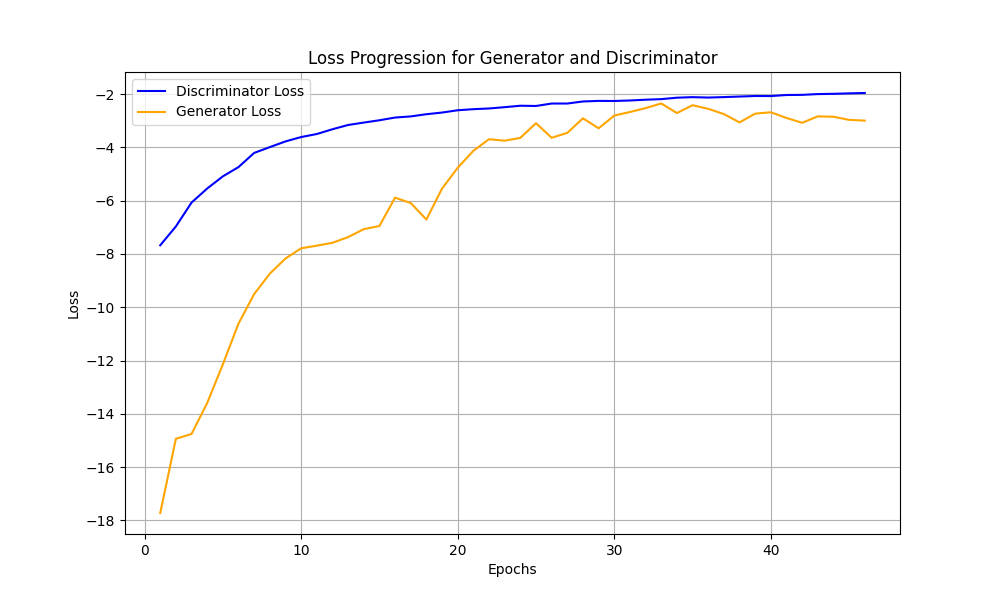
\includegraphics[width=80mm]{loss_D_G.png}
\caption{Discriminator Loss during Training (WGAN)}
\end{figure}
\\
In general , especially because the problem has been simplified with respect 
to the previous one , after only 50 epochs we can appreciate good result in term of 
reconstruction of image related to the MNIST datasets .
And thanks to the gradient penalty term we can generalize the enough to obtain 
a good reconstruction also on "zero-shot" data coming from the same dataset . 
\\
The visual results of the model's performance after various epochs are shown below. 
As it is possible to observe, the reconstructions generated by the "Generator" become 
increasingly coherent with the noise given as input as the epochs increase.

\begin{figure}[h!]
    \centering
    \caption{Grid of generated images at different epochs}
    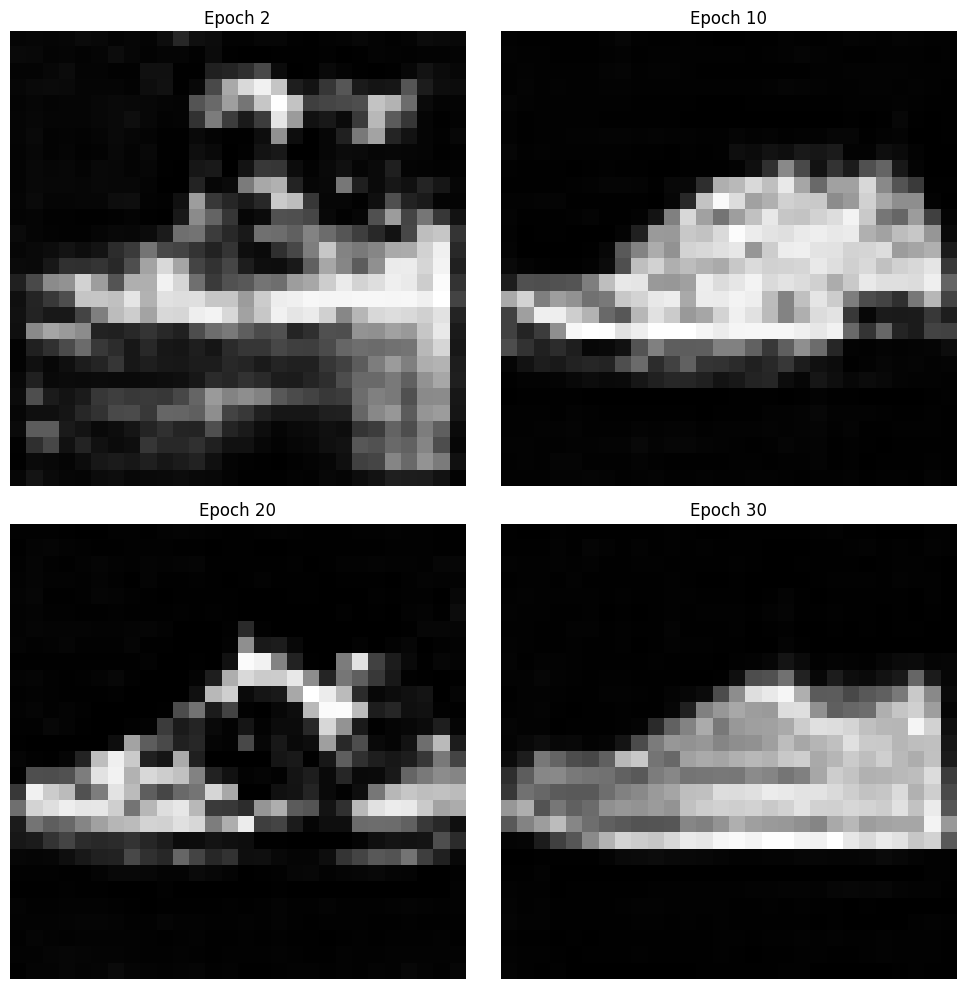
\includegraphics[width=0.4\textwidth]{images/Epochs.png}
    \label{fig:grid_plot}
\end{figure}




%----------------------------------------------------------------------------------------
% REFERENCE LIST
%----------------------------------------------------------------------------------------

% \begin{thebibliography}{10} % 10 is a random guess of the total number of references
% \bibitem{MG} Goossens, M., Mittelbach, F., Samarin, \emph{A LaTeX
% Companion}, Addison-Wesley, Reading, MA, 1994.
% \end{thebibliography}
%----------------------------------------------------------------------------------------
\end{document}